\documentclass[12pt]{report}
\usepackage[utf8]{inputenc}
\usepackage[T2A]{fontenc}
\usepackage[russian]{babel}

\usepackage{amsmath,amsfonts,amssymb,amsthm,mathtools}
\DeclarePairedDelimiter\abs{\lvert}{\rvert}

\usepackage{pgfplots}
\usepackage{filecontents}
\usepackage{indentfirst}
\usepackage{eucal}
\usepackage{enumitem}
% Для \abs{}
\usepackage{commath}
\usepackage{float}
\frenchspacing

% Для нормальных переносов
\sloppy

\usetikzlibrary{datavisualization}
\usetikzlibrary{datavisualization.formats.functions}

\usepackage[left=2cm,right=2cm, top=2cm,bottom=2cm,bindingoffset=0cm]{geometry}
% Для измененных титулов глав:
\usepackage{titlesec, blindtext, color} % подключаем нужные пакеты
\definecolor{gray75}{gray}{0.75} % определяем цвет
\newcommand{\hsp}{\hspace{20pt}} % длина линии в 20pt
% titleformat определяет стиль
\titleformat{\chapter}[hang]{\Huge\bfseries}{\thechapter\hsp\textcolor{gray75}{|}\hsp}{0pt}{\Huge\bfseries}

% plot
\usepackage{xcolor}
\usepackage{stmaryrd}
\usepackage{wasysym}
\usetikzlibrary{datavisualization}
\usetikzlibrary{datavisualization.formats.functions}

% листинги
\usepackage{listings}
\usepackage{graphicx}
\usepackage{caption}
\usepackage{textcomp}
\lstset{
    language = Python,
    basicstyle=\small\sffamily,
    numbers=left,
    numberstyle=\tiny,
    stepnumber=1,
    numbersep=5pt,
    showspaces=false,
    showstringspaces=false,
    showtabs=false,
    frame=single,
    tabsize=2,
    captionpos=t,
    breaklines=true,
    breakatwhitespace=false,
    escapeinside={\#*}{*)},
    literate=	{а}{{\selectfont\char224}}1
			    {б}{{\selectfont\char225}}1
			    {в}{{\selectfont\char226}}1
			    {г}{{\selectfont\char227}}1
			    {д}{{\selectfont\char228}}1
			    {е}{{\selectfont\char229}}1
			    {ё}{{\"e}}1
			    {ж}{{\selectfont\char230}}1
			    {з}{{\selectfont\char231}}1
			    {и}{{\selectfont\char232}}1
			    {й}{{\selectfont\char233}}1
			    {к}{{\selectfont\char234}}1
			    {л}{{\selectfont\char235}}1
			    {м}{{\selectfont\char236}}1
			    {н}{{\selectfont\char237}}1
			    {о}{{\selectfont\char238}}1
			    {п}{{\selectfont\char239}}1
			    {р}{{\selectfont\char240}}1
			    {с}{{\selectfont\char241}}1
			    {т}{{\selectfont\char242}}1
			    {у}{{\selectfont\char243}}1
			    {ф}{{\selectfont\char244}}1
			    {х}{{\selectfont\char245}}1
			    {ц}{{\selectfont\char246}}1
			    {ч}{{\selectfont\char247}}1
			    {ш}{{\selectfont\char248}}1
			    {щ}{{\selectfont\char249}}1
			    {ъ}{{\selectfont\char250}}1
			    {ы}{{\selectfont\char251}}1
			    {ь}{{\selectfont\char252}}1
			    {э}{{\selectfont\char253}}1
			    {ю}{{\selectfont\char254}}1
			    {я}{{\selectfont\char255}}1
			    {А}{{\selectfont\char192}}1
			    {Б}{{\selectfont\char193}}1
			    {В}{{\selectfont\char194}}1
			    {Г}{{\selectfont\char195}}1
			    {Д}{{\selectfont\char196}}1
			    {Е}{{\selectfont\char197}}1
			    {Ё}{{\"E}}1
			    {Ж}{{\selectfont\char198}}1
			    {З}{{\selectfont\char199}}1
			    {И}{{\selectfont\char200}}1
			    {Й}{{\selectfont\char201}}1
			    {К}{{\selectfont\char202}}1
			    {Л}{{\selectfont\char203}}1
			    {М}{{\selectfont\char204}}1
			    {Н}{{\selectfont\char205}}1
			    {О}{{\selectfont\char206}}1
			    {П}{{\selectfont\char207}}1
			    {Р}{{\selectfont\char208}}1
			    {С}{{\selectfont\char209}}1
			    {Т}{{\selectfont\char210}}1
			    {У}{{\selectfont\char211}}1
			    {Ф}{{\selectfont\char212}}1
			    {Х}{{\selectfont\char213}}1
			    {Ц}{{\selectfont\char214}}1
			    {Ч}{{\selectfont\char215}}1
			    {Ш}{{\selectfont\char216}}1
			    {Щ}{{\selectfont\char217}}1
			    {Ъ}{{\selectfont\char218}}1
			    {Ы}{{\selectfont\char219}}1
			    {Ь}{{\selectfont\char220}}1
			    {Э}{{\selectfont\char221}}1
			    {Ю}{{\selectfont\char222}}1
			    {Я}{{\selectfont\char223}}1
			    {№}{{\selectfont N}}1
}
\captionsetup[lstlisting]{justification=raggedright, singlelinecheck=off}

\addto\captionsrussian{% Replace "english" with the language you use
	\renewcommand{\contentsname}%
	{Содержание	}%
}

\begin{document}
	% Титульник
\thispagestyle{empty}
\begin{titlepage}
	\noindent \begin{minipage}{0.15\textwidth}
		
\includegraphics[width=\linewidth]{img/b-logo}
	\end{minipage}
	\noindent\begin{minipage}{0.9\textwidth}
		\centering
		\textbf{Министерство науки и высшего образования Российской Федерации}\\
		\textbf{Федеральное государственное бюджетное образовательное учреждение высшего образования}\\
		\textbf{~~~«Московский государственный технический университет имени Н.Э.~Баумана}\\
		\textbf{(национальный исследовательский университет)»}\\
		\textbf{(МГТУ им. Н.Э.~Баумана)}
	\end{minipage}
	
	\noindent\rule{18cm}{3pt}
	\newline\newline
	\noindent ФАКУЛЬТЕТ $\underline{\text{«Информатика и системы управления»}}$ \newline\newline
	\noindent КАФЕДРА $\underline{\text{«Программное обеспечение ЭВМ и информационные технологии»}}$\newline\newline\newline\newline\newline
	
	
	\begin{center}
		\noindent\begin{minipage}{1.3\textwidth}
			\centering
			\Large\textbf{  Отчет по лабораторной работе №3}\newline
			\textbf{по дисциплине "Анализ алгоритмов"}\newline\newline
		\end{minipage}
	\end{center}
	
	\noindent\textbf{Тема} $\underline{\text{Сравнительный анализ алгоритмов сортировки}}$\newline\newline
	\noindent\textbf{Студент} $\underline{\text{Шацкий Р.Е.}}$\newline\newline
	\noindent\textbf{Группа} $\underline{\text{ИУ7-55Б}}$\newline\newline
	\noindent\textbf{Оценка (баллы)} $\underline{\text{~~~~~~~~~~~~~~~~~~~~~~~~~~~}}$\newline\newline
	\noindent\textbf{Преподаватели} $\underline{\text{Волкова Л.Л., Строганов Ю.В.}}$\newline\newline\newline
	
	\begin{center}
		\vfill
		Москва~---~\the\year
		~г.
	\end{center}
\end{titlepage}
	\pagenumbering{arabic}
	\newpage
	\tableofcontents
    \chapter*{Введение}
    \addcontentsline{toc}{chapter}{Введение}
    
    Одной из частых задач в программировании является задача доступа к некоторому набору элементов. Например, обычные списки (массивы) представляют собой набор пронумерованных элементов, то есть для обращения к какому-либо элементу списка необходимо указать его номер. Номер элемента в списке однозначно идентифицирует сам элемент.
    
    Но идентифицировать данные по числовым номерам не всегда оказывается удобно. Например, маршруты поездов в России идентифицируются численно-буквенным кодом (число и одна цифра), также численно-буквенным кодом идентифицируются авиарейсы, то есть для хранения информации о рейсах поездов или самолетов в качестве идентификатора удобно было бы использовать не число, а текстовую строку.
    
    Структура данных, позволяющая идентифицировать ее элементы не по числовому индексу, а по произвольному, называется словарем или ассоциативным массивом. Каждый элемент словаря состоит из двух объектов: ключа и значения. 
    В жизни широко распространены словари, например, привычные бумажные словари (толковые, орфографические, лингвистические). В них ключом является слово-заголовок статьи, а значением — сама статья. Для того, чтобы получить доступ к статье, необходимо указать слово-ключ.
    
    Другой пример словаря, как структуры данных — телефонный справочник. В нем ключом является имя, а значением — номер телефона. И словарь, и телефонный справочник хранятся так, что легко найти элемент словаря по известному ключу (например, если записи хранятся в алфавитном порядке ключей, то легко можно найти известный ключ, например, бинарным поиском), но если ключ неизвестен, а известно лишь значение, то поиск элемента с данным значением может потребовать последовательного просмотра всех элементов словаря.
    
    Особенностью ассоциативного массива является его динамичность: в него можно добавлять новые элементы с произвольными ключами и удалять уже существующие элементы. При этом размер используемой памяти пропорционален размеру ассоциативного массива. Доступ к элементам ассоциативного массива выполняется хоть и медленнее, чем к обычным массивам, но в целом довольно быстро.
    
    Словари нужно использовать в следующих случаях.
    \begin{enumerate}
    	\item Подсчет числа каких-то объектов. В этом случае нужно завести словарь, в котором ключами являются объекты, а значениями — их количество.
    	\item Хранение каких-либо данных, связанных с объектом. Ключи — объекты, значения — связанные с ними данные.
    	\item Установка соответствия между объектами (например, “родитель—потомок”). Ключ — объект, значение — соответствующий ему объект.
    	\item Если нужен обычный массив, но при этом максимальное значение индекса элемента очень велико, но при этом будут использоваться не все возможные индексы (так называемый “разреженный массив”), то можно использовать ассоциативный массив для экономии памяти.
    \end{enumerate}
    
    Целью данной лабораторной работы является изучение и сравнение алгоритмов поиска по словарю.
    
    Для достижения поставленной цели необходимо выполнить следующие задачи:
    
    \begin{itemize}
    	\item изучить существующие алгоритмы поиска по словарю;
    	\item определить требования к программе для решения задачи поиска по словарю;
    	\item описать структуры данных;
    	\item определить классы эквивалентности для тестирования;
    	\item определить тестовые данные;
    	\item осуществить выбор средств реализации;
    	\item реализовать алгоритмы программно;
    	\item исследовать время работы алгоритмов;
    	\item сравнить время работы алгоритмов и сделать соответствующие выводы.
    \end{itemize}
    
    \chapter{Аналитическая часть}
    
    В данном разделе будут рассмотрены существующие алгоритмы поиска по словарю и 
    определены требования к разрабатываемой программе.
    
    \section{Алгоритмы поиска по словарю}
    
    Для решения задачи поиска по словарю можно использовать следующие алгоритмы:
    \begin{itemize}
    	\item алгоритм полного перебора;
    	\item алгоритм двоичного поиска;
    	\item алгоритм частотного анализа.
    \end{itemize}
    
    Рассмотрим каждый из них.
    
    \subsection{Алгоритм полного перебора}
    
    Алгоритмом полного перебора называют метод решения задачи, при котором по очереди рассматриваются все возможные варианты исходного набора данных. В случае словарей будет произведен последовательный перебор элементов словаря до тех пор, пока не будет найден необходимый. Сложность такого алгоритма зависит от количества всех возможных решений, а время работы может стремиться к экспоненциальному.
    
    Пусть алгоритм нашел элемент на первом сравнении. Тогда, в лучшем случае, будет затрачено $k_0 + k_1$ операций, на втором -- $k_0 + 2k_1$, на $N$ -- $k_0 + Nk_1$. тогда, средняя трудоемкость может быть рассчитано по формуле \eqref{eq:brute}, где $\Omega$ - множество всех возможных случаев.
    
    \begin{equation}
    	\label{eq:brute}
    	\sum_{i \in \Omega} p_i t_i = (k_0 + k_1) \frac{1}{N + 1} + (k_0 + 2k_1) * \frac{1}{N + 1} + \dots + (k_0 + Nk_1) * \frac{1}{N + 1} 
    \end{equation}
    Из \eqref{eq:brute}, сгруппировав слагаемые, получим итоговую формулу для расчета средней трудоемкости работы алгоритма:
    
    \begin{equation}
    	k_0 + k1(\frac{N}{N + 1} + \frac{N}{2}) = k_0 + k1(1 + \frac{N}{2} - \frac{1}{N + 1}) 
    \end{equation}
    
    \subsection{Алгоритм двоичного поиска}
    Данный алгоритм применяется к заранее упорядоченным словарям. Процесс двоичного поиска можно описать при помощи шагов:
    \begin{itemize}
    	\item сравнить значение ключа, находящегося в середине рассматриваемого интервала (изначально -- весь словарь), с данным;
    	\item в случае, если значение меньше (в контексте типа данных) данного, продолжить поиск в левой части интервала, в обратном - в правой;
    	\item продолжать до тех пор, пока найденное значение не будет равно данному или длина интервала не станет равной нулю (означает отсутствие искомого ключа в словаре).
    \end{itemize}
    Использование данного алгоритма в для поиска в словаре в любом из случаев будет иметь трудоемкость равную $O(log_2(N))$ \cite{2}. Несмотря на то, что в среднем и худшем случаях данный алгоритм работает быстрее алгоритма полного перебора, стоит отметить, что предварительная сортировка больших данных требует дополнительных затрат по времени и может оказать серьезное действие на время работы алгоритма. Тем не менее, при многократном поиске по одному и тому же словарю, применение алгоритм сортировки понадобится всего один раз.
    
    \subsection{Алгоритм частотного анализа}
    Алгоритм частотного анализа строит частотный анализ полученного словаря. Чтобы провести частотный анализ, нужно взять первый элемент каждого значения в словаре по ключу и подсчитать частотную характеристику, т.е. сколько раз этот элемент встречался в качестве первого. По полученным данным словарь разбивается на сегменты так, что все записи с одинаковым первым элементом оказываются в одном сегменте.
    
    Сегменты упорядочиваются по значению частотной характеристики таким образом, чтобы к элементу с наибольшим значением характеристики был предоставлен самый быстрый доступ.
    
    Затем каждый из сегментов упорядочивается по значению. Это необходимо для реализации бинарного поиска, который обеспечит эффективный поиск в сегмента при сложности $O(nlog(n))$ таким образом, сначала выбирается нужный сегмент, а затем в нем проводится бинарный поиск  нужного элемента. Средняя трудоемкость при длине алфавита $M$ может быть рассчитана по формуле \eqref{eq:freq}.
    
    \begin{equation}
    	\sum_{i \in [1, M]} (f_{select_i} + f_{search_i})
    	\label{eq:freq}
    \end{equation}
    
    \section{Словарь}
    В качестве словаря предлагается использовать домен - "Модели телефонов".

 	Сущностью является модель телефона и компания-производитель, записанные в одной строке через разделитель.
    
    \section{Вывод}
    В данном разделе были рассмотрены алгоритмы для решения задачи поиска по словарю.
    
    Для изучения данных алгоритмов необходимо реализовать программное обеспечение, выполняющее следующие функциональные требования:
    \begin{enumerate}
    	\item На вход подается словарь из записей, вида \{model: string, value: string\} для поиска по нему и ключ для поиска в словаре.
    	\item Выходными данными является найденная в словаре запись для каждого из реализуемых алгоритмов.
    \end{enumerate}

	\section*{Вывод}
	В данном разделе были описаны принципы работы муравьиного алгоритма и алгоритма полного перебора.
	Выдвинуты требования к разрабатываемому ПО: входные данные, выходные данные и наличие обработки некорректного ввода.
	\newpage
	
	\chapter{Конструкторская часть}
	
	В данном разделе будут описаны структуры данных и алгоритмы для решения задачи поиска по словарю,
	которые будут реализованы в программе.
	Кроме того, будут определены классы эквивалентности для тестирования.
	
	\section{Схемы алгоритмов}
	
	На рисунках \ref{fig:alg1}, \ref{fig:alg2} и \ref{fig:alg3} представлены схемы использованных алгоритмов.
	
	\begin{figure}[H]
		\begin{center}
			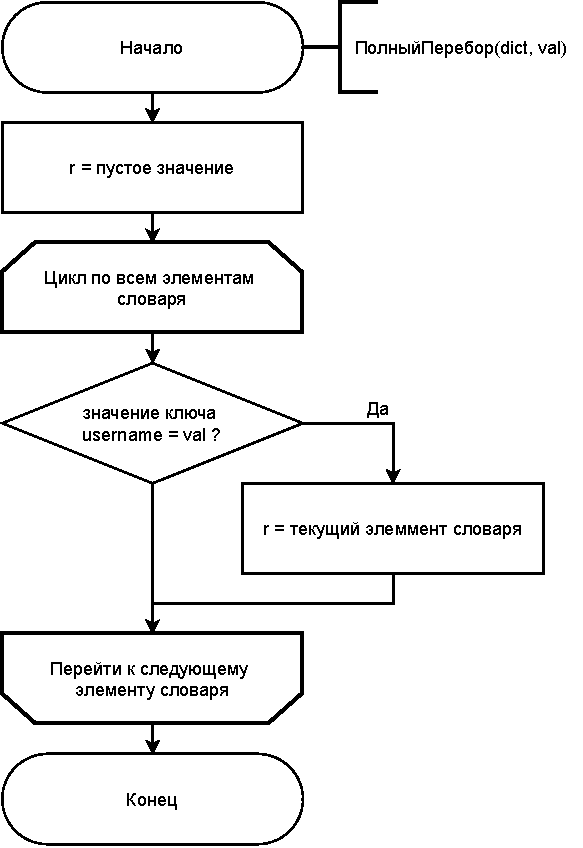
\includegraphics[scale=0.8]{img/brute_scheme.pdf}
			\caption{Схема алгоритма поиска с полным перебором.}
			\label{fig:alg1}
		\end{center}
	\end{figure}
	
	\begin{figure}[H]
		\begin{center}
			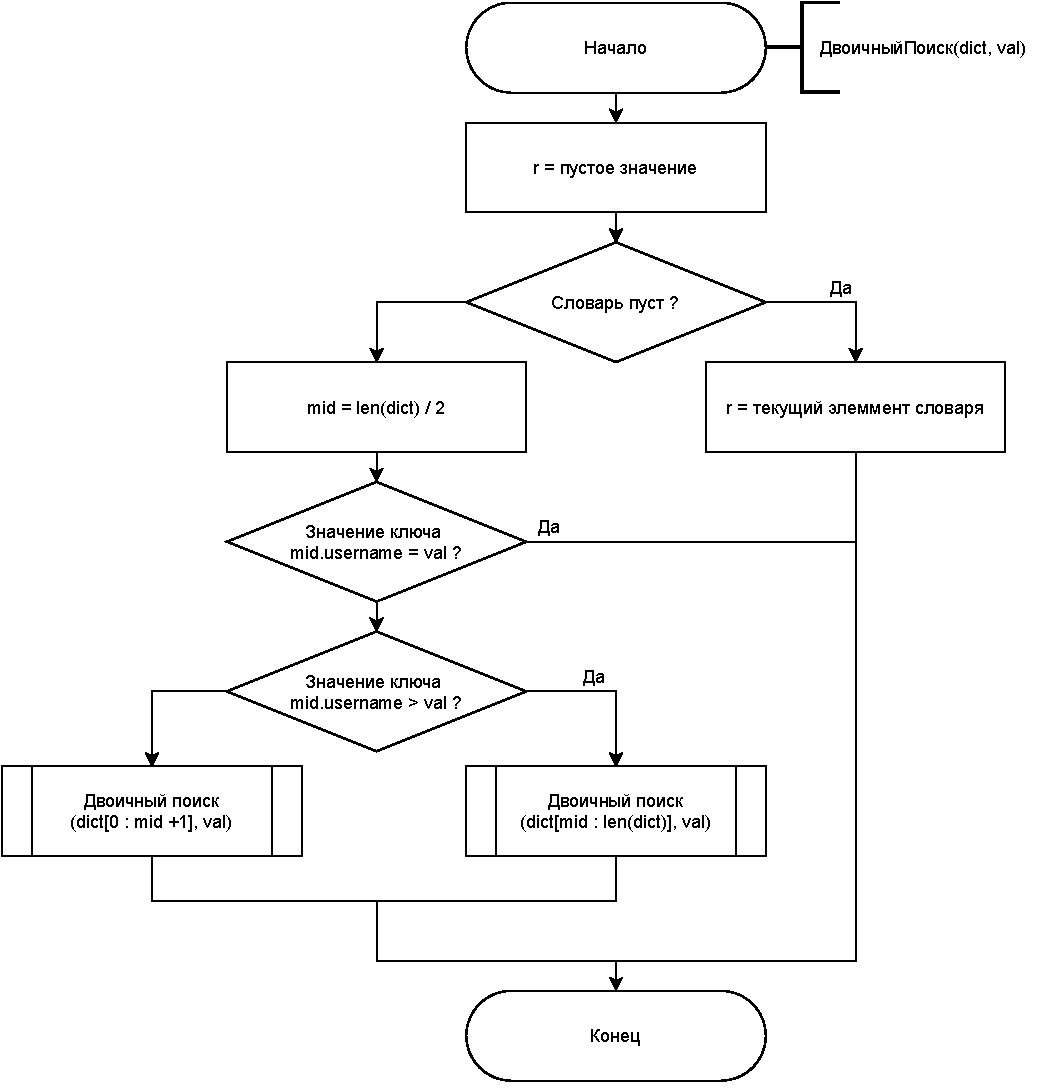
\includegraphics[scale=0.8]{img/bin_scheme.pdf}
			\caption{Схема алгоритма с бинарным поиском.}
			\label{fig:alg2}
		\end{center}
	\end{figure}
	
	\newpage
	\begin{figure}[H]
		\begin{center}
			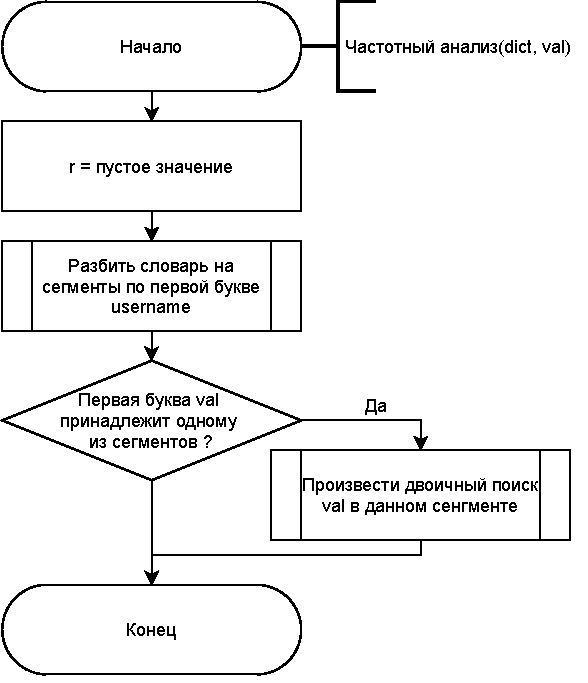
\includegraphics[scale=0.8]{img/freq_scheme.pdf}
			\caption{Схема алгоритма с частотным анализом.}
			\label{fig:alg3}
		\end{center}
	\end{figure}
	
	\section{Структуры данных}

	Для реализации алгоритмов необходимо использовать следующие структуры данных:
	
	\begin{enumerate}
		\item Структура, описывающая ассоциативный массив с ключами типа string.
		\item Структура, описывающая сегмент частотного анализа ассоциативного массива.
	\end{enumerate}
	
	Для реализации структуры, описывающей ассоциативный массив, будет использован словарь (dict).
	
	Для реализации структуры, описывающей сегмент частотного анализа, будет использован следующий набор полей:
	\begin{enumerate}
		\item \texttt{l} -- строка, содержащая признак сегмента -- букву из используемого алфавита;
		\item \texttt{cnt} -- частотная характеристика для данного сегмента;
		\item \texttt{darr} -- ассоциативный массив, содержащий записи, соответствующие данному сегменту.
	\end{enumerate}
	
	\section{Тестирование}
	Для детального тестирования программы, можно выделить несколько классов эквивалентности:
	\begin{itemize}
		\item ключ отсутсвует в словаре;
		\item ключ является первым элементом словаря;
		\item ключ является последним элементом словаря;
		\item ключ является произвольным элементом словаря.
	\end{itemize}
	
	\section{Структура программного обеспечения}
	На рисунке \ref{fig:idef0} показана функциональная схема программного обеспечения.
	
	\begin{figure}[H]
		\begin{center}
			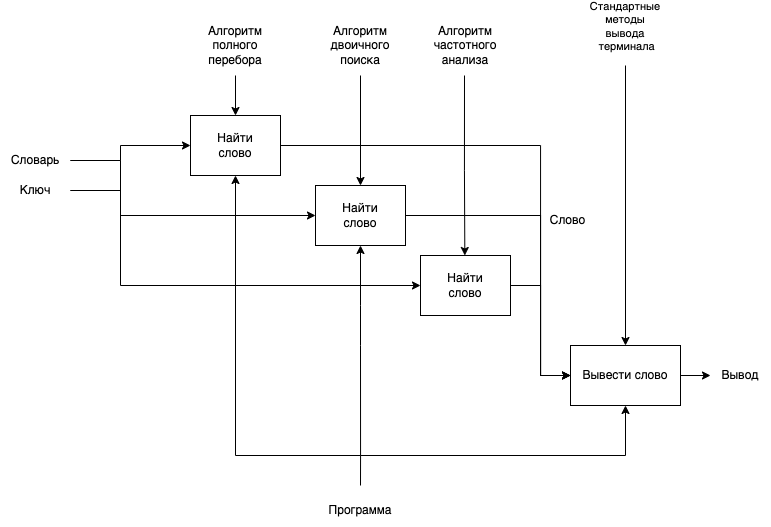
\includegraphics[scale=0.5]{img/idef0.png}
			\caption{Функциональная схема программного обеспечения, idef0}
			\label{fig:idef0}
		\end{center}
	\end{figure}
	
	\section{Вывод}
	В данном разделе мы исследовали алгоритмы и структуры данных, которые будут использованы в программе,
	определили классы эквивалентности для тестирования и определили структуру программного обеспечения.
	
	\chapter{Технологическая часть}
	В данном разделе будет осуществлен выбор средств реализации,
	разобран код реализованных алгоритмов и определены тестовые данные.
	
	\section{Выбор средств реализации}
	В качестве средства реализации было решено использовать язык программирования Python, так как уже имеется опыт работы с библиотеками и инструмантами языка, которые позволяют реализовать и провести исследования алгоритмов.
	
	Для замера времени выполнения использовалась функция time() из библиотеки time.
	
	\section{Сведения о модулях программы}
	Программа состоит из следующих модулей:
	\begin{itemize}
		\item main.py - модуль с тестами и пользовательским вводом;
		\item search.py - модуль с реализованными классами, наследованными от BaseSearcher, с методами для выполнения поиска в словаре.
	\end{itemize}
	
	\newpage
	\section{Листинг кода реализованных алгоритмов}
	
	В листингах \ref{lst:1}, \ref{lst:2} и \ref{lst:3} представлен код используемых алгоритмов.
	
	\begin{lstlisting}[label={lst:1},caption= Алгоритм полного перебора.]
		class SimpleSearcher(BaseSearcher):
			def __init__(self, _dict: dict[str, str]):
				super().__init__(_dict)
			
			def search(self, key: str) -> str or None:
				for item in self._dict.items():
					if item[0] == key:
						return item[1]
					return None
	\end{lstlisting}
	
	\begin{lstlisting}[label={lst:2},caption=Алгоритм бинарного поиска.]
		class BinarySearcher(BaseSearcher):
			def __init__(self, _dict: dict[str, str]):
				super().__init__(_dict)

			def search(self, key: str) -> str or None:
				return BinarySearcher._search(key, self._dict)

			@staticmethod
			def _search(key: str, _dict: dict[str, str]) -> str or None:
				"""
				_dict must be already sorted (ascending)

				:param key: key to find in _dict
				:param _dict: ascending sorted dictionary
				:return: _dict value by key
				"""
				sorted_keys = list(_dict.keys())
				sorted_values = list(_dict.values())

				down_limit: int = 0
				up_limit: int = len(_dict) - 1
				center_i: int = up_limit // 2

				while sorted_keys[center_i] != key and down_limit < up_limit:
					if key > sorted_keys[center_i]:
						down_limit = center_i + 1
					else:
						up_limit = center_i - 1
					center_i = int((down_limit + up_limit) / 2)

				if down_limit >= up_limit:
					return None
				return sorted_values[center_i]
	\end{lstlisting}
	
	\newpage
	\begin{lstlisting}[label={lst:3},caption=Алгоритм частотного анализа.]
		class CombinedSearcher(BaseSearcher):
			def __init__(self, _dict: dict[str, str]):
				super().__init__(_dict)
				self.segments: [dict] = self.frequency_analysis()

			def frequency_analysis(self):
				# Сколько раз встречается первый символ каждого ключа  _dict
				frequency_dict: dict[str, int] = {}
				for key in self._dict.keys():
					if key[0] in frequency_dict.keys():
						frequency_dict[key[0]] += 1
					else:
						frequency_dict[key[0]] = 1
				segmented_list: [dict] = []
				for key_letter in frequency_dict.keys():
					keys = {'letter': key_letter, 'count': frequency_dict[key_letter], 'dict': {}}

					for key in self._dict.keys():
						if key[0] == key_letter:
							keys['dict'][key] = self._dict[key]
					# сортировка словаря по ключу
					keys['dict'] = dict(sorted(keys['dict'].items()))

					segmented_list.append(keys)

				segmented_list.sort(key=lambda value: value['count'], reverse=True)
				return segmented_list

			def search(self, key: str) -> str or None:
				"""
				_dict can be any dictionary

				:param key: key to find in _dict
				:param _dict: any dictionary
				:return: _dict value by key
				"""
				found_dict = {}
				for i in range(len(self.segments)):
					if self.segments[i]['letter'] == key[0]:
						found_dict = self.segments[i]['dict']
						break

				if len(found_dict) == 0:
					return None

				return BinarySearcher._search(key, found_dict)
	\end{lstlisting}
	
	
	\section{Тесты для проверки корректности программы}
	В рамках данной лабораторной работы будет проведено функциональное тестирование реализованного программного обеспечения.

	Тестирование проводилось на словаре, содержащем следующие записи:
	\begin{itemize}
		\item \texttt{\{key: "C1 --- Nokia"; value:"successfully found"\}};
		\item \texttt{\{key: "2.3 --- Nokia"; value:"successfully found"\}};
		\item \texttt{\{key: "7.2 --- Nokia"; value:"successfully found"\}}.
	\end{itemize}
	
	В Таблице \ref{tbl:tests} приведены соответствующие тесты.
	
	\begin{table}[H]
		\small
		\begin{center}
			\captionsetup{justification=raggedright, singlelinecheck=false}
			\caption{Таблица тестов}
			\label{tbl:tests}
			\begin{tabular}{|c|l|l|}
				\hline
				\bfseries Ключ & \bfseries Результат & \bfseries Ожидаемое значение \\ \hline
				\texttt{C1 --- Nokia} & "successfully found" & "successfully found" \\\hline
				\texttt{7.2 --- Nokia} & "successfully found" & "successfully found" \\\hline
				\texttt{asd} & \bfseries None & \bfseries None \\\hline
			\end{tabular}
		\end{center}
	\end{table}
	
	При проведении функционального тестирования, результаты работы программы совпали с ожидаемыми. Таким образом, функциональное тестирование пройдено успешно.
	
	\section{Вывод}
	В данном разделе было выбрано средство реализации, разобран код реализованных алгоритмов и определены тестовые данные.
	\newpage
	
	\chapter{Экспериментальная часть}
	
	\paragraph{}
	В данном разделе будет исследовано время работы алгоритмов:
	\begin{itemize}
		\item алгоритм полного перебора;
		\item алгоритм двоичного поиска;
		\item алгоритм частотного анализа.
	\end{itemize}
	
	\section{Технические характеристики}
	Технические характеристики устройства, на котором выполнялось тестирование:
	\begin{itemize}
		\item операционная система: Windows~\cite{windows} 10 64-bit;
		\item оперативная память: 16 Гб;
		\item процессор: Intel(R) Core(TM) i5-7600 CPU @ 3.50GHz \cite{i5}.
	\end{itemize}
	
	\section{Временные характеристики}
	
	В реализованном программном обеспечении особый интерес представляет количество сравнений, необходимое для нахождения записи в словаре по ключу, так как это характеристика прямо пропорциональна времени работы алгоритма. Поэтому, будет проводиться анализ количества сравнений каждого из ключей словаря в словаре и время поиска ключа не находящегося в словаре. Для большей наглядности число записей в словаре возьмем равным $2000$. 
	
	Поиск будет производиться каждым алгоритмом по отдельности, после чего будут представлены соответствующие гистограммы. Отметим, что, в общем случае, распределение носит достаточно "случайный"\ характер, так как исходный массив не обязательно является упорядоченным. В связи с этим, каждая из построенных гистограмм будет продублирована второй, отображающей данные по убыванию числа сравнений.
	
	\subsection{Алгоритм полного перебора}
	
	В данном алгоритме зависимости числа сравнений от количества элементов является линейной. На пример, для обнаружения первого элемента понадобится 1 сравнение, для 2ого -- 2, а для $N$-ого -- $N$.  В связи с этим, поиск последнего элемента в массиве потребует $N$ сравнений. 
	
	\begin{figure}[H]
		\begin{center}
			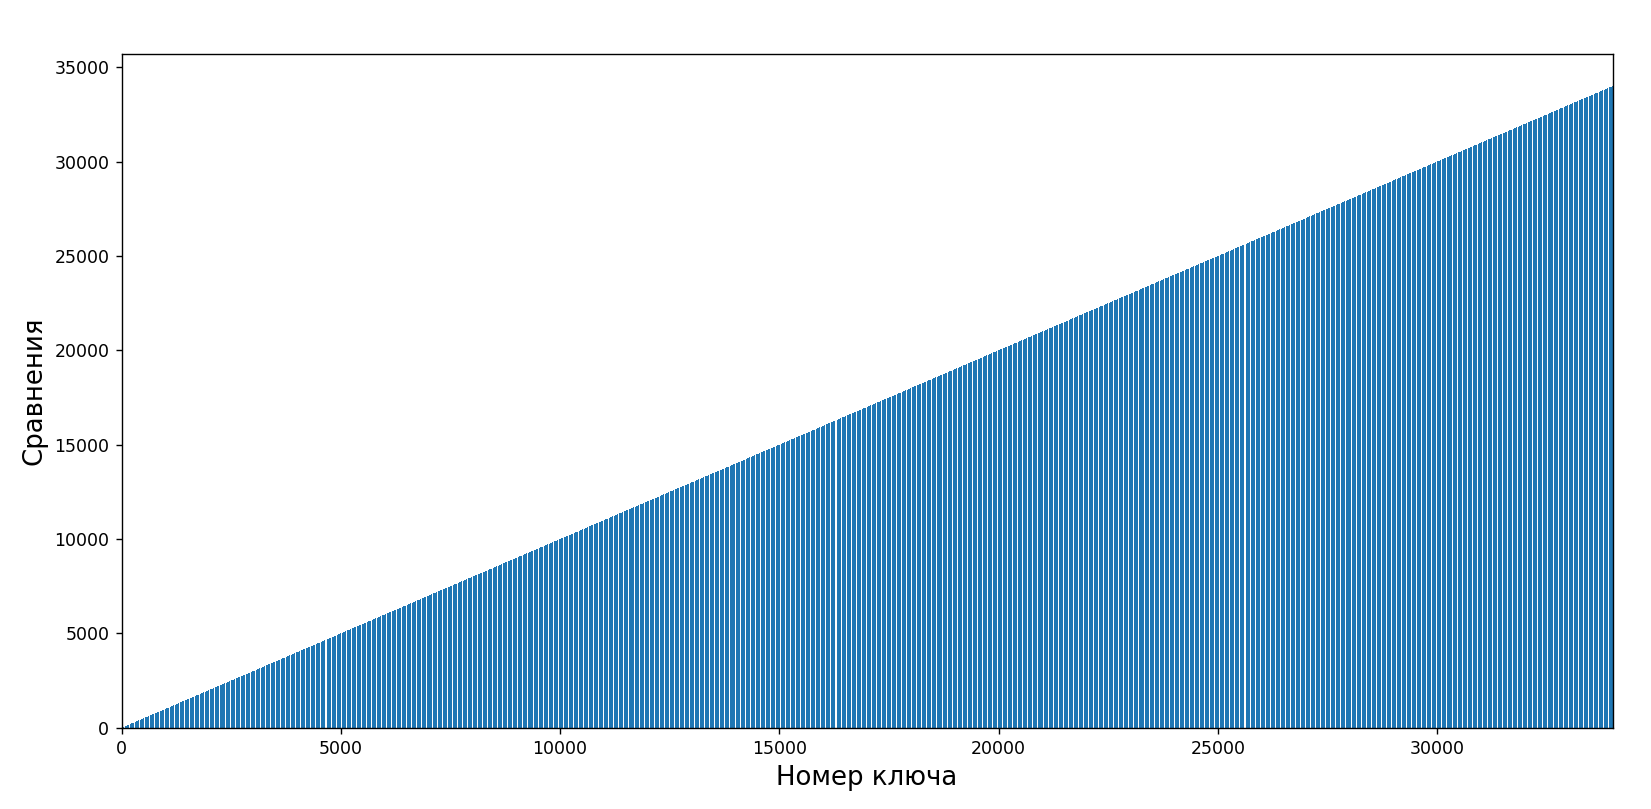
\includegraphics[width=0.8\linewidth]{img/plunc_keys}
			\caption{Число сравнений для нахождения полным перебором.}
			\label{img:brute}
		\end{center}
	\end{figure}
	
	На Рисунке \ref{img:brute} видна линейная зависимость числа сравнений от положения элемента в массиве.
	
	\begin{figure}[H]
		\begin{center}
			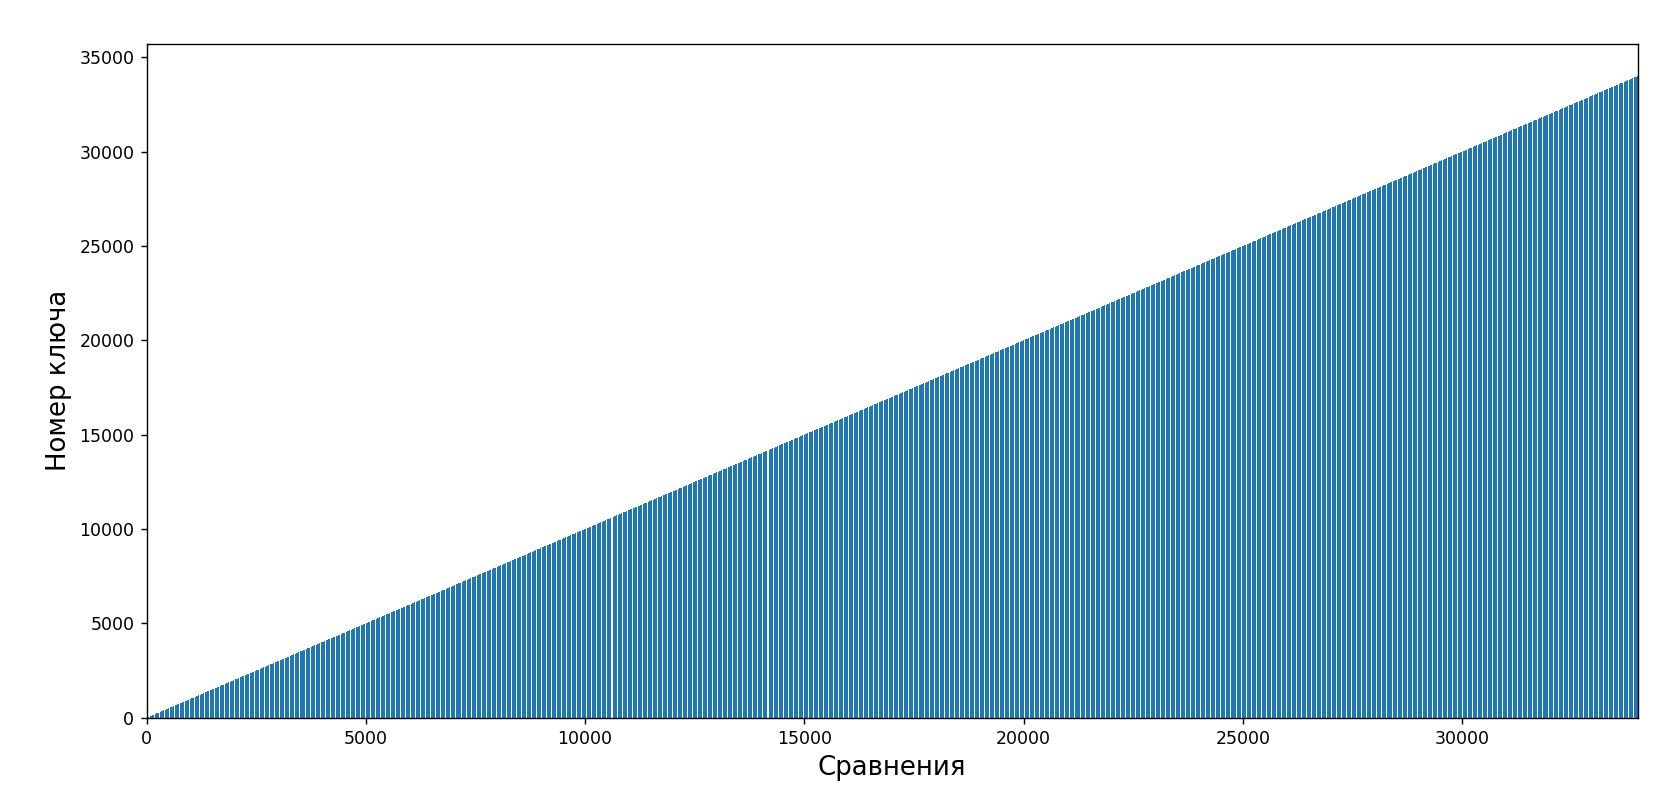
\includegraphics[width=0.8\linewidth]{img/plunc_comp}
			\caption{Число сравнений для нахождения полным перебором по убыванию.}
			\label{img:brute_sorted}
		\end{center}
	\end{figure}
	
	\subsection{Алгоритм бинарного поиска}
	
	В данном алгоритме сложность поиска равна $O(log(N))$, в связи с этим, на общей гистограмме будет наблюдаться достаточно произвольное распределение, зависящее от входного массива.
	
	\begin{figure}[H]
		\begin{center}
			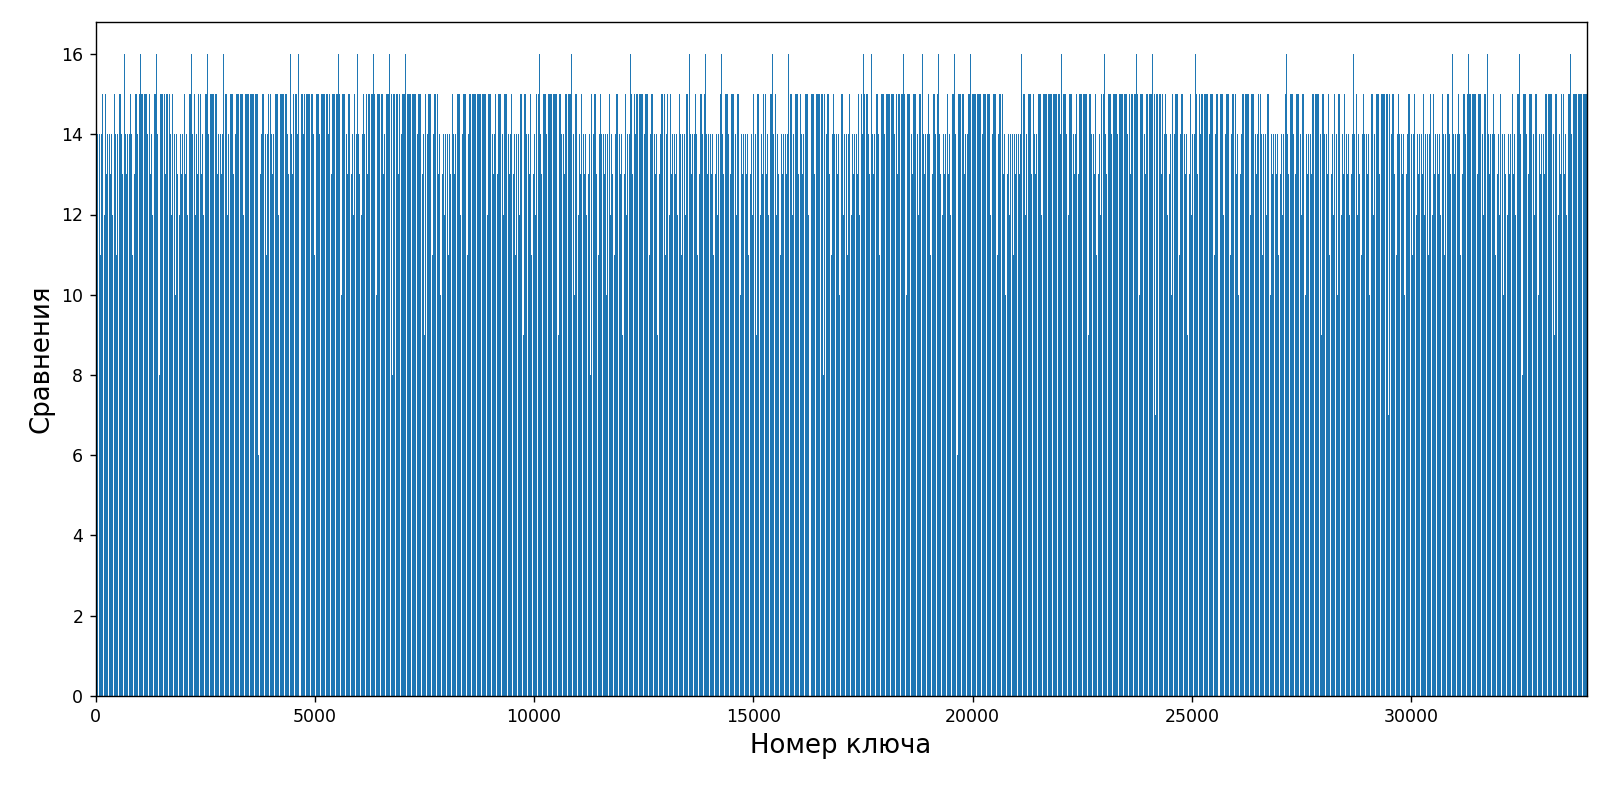
\includegraphics[width=0.8\linewidth]{img/bin_keys}
			\caption{Число сравнений для нахождения бинарным поиском.}
			\label{img:bin}
		\end{center}
	\end{figure}
	
	На Рисунке \ref{img:bin} не наблюдается явной зависимости числа сравнений для поиска элемента от его значения. В связи с этим, стоит упорядочить элементы по числу сравнений и построить вторую гистограмму.
	
	\begin{figure}[H]
		\begin{center}
			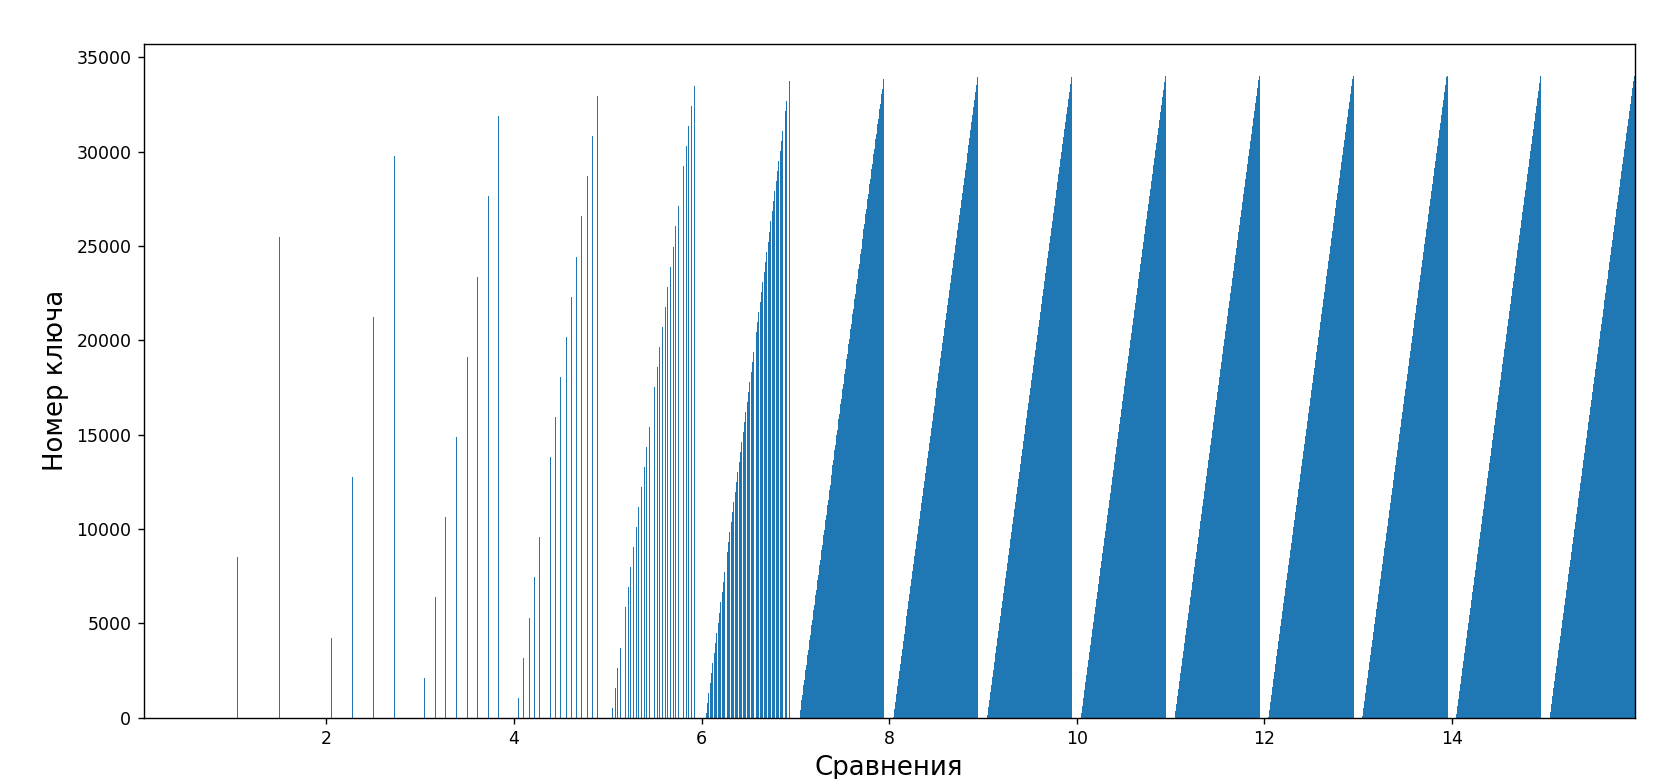
\includegraphics[width=0.8\linewidth]{img/bin_comp.png}
			\caption{Число сравнений для нахождения бинарным поиском по убыванию.}
			\label{img:bin_sorted}
		\end{center}
	\end{figure}
	
	\subsection{Алгоритм частотного анализа}
	
	В данном алгоритме сложность поиска зависит не только от положения в отсортированном сегменте, но и от размера используемого словаря, так как поиск в нем осуществляется полным перебором. Тем не менее, в среднем случае это не должно оказывать серьезного действия на число требуемых сравнений.
	
	\begin{figure}[H]
		\begin{center}
			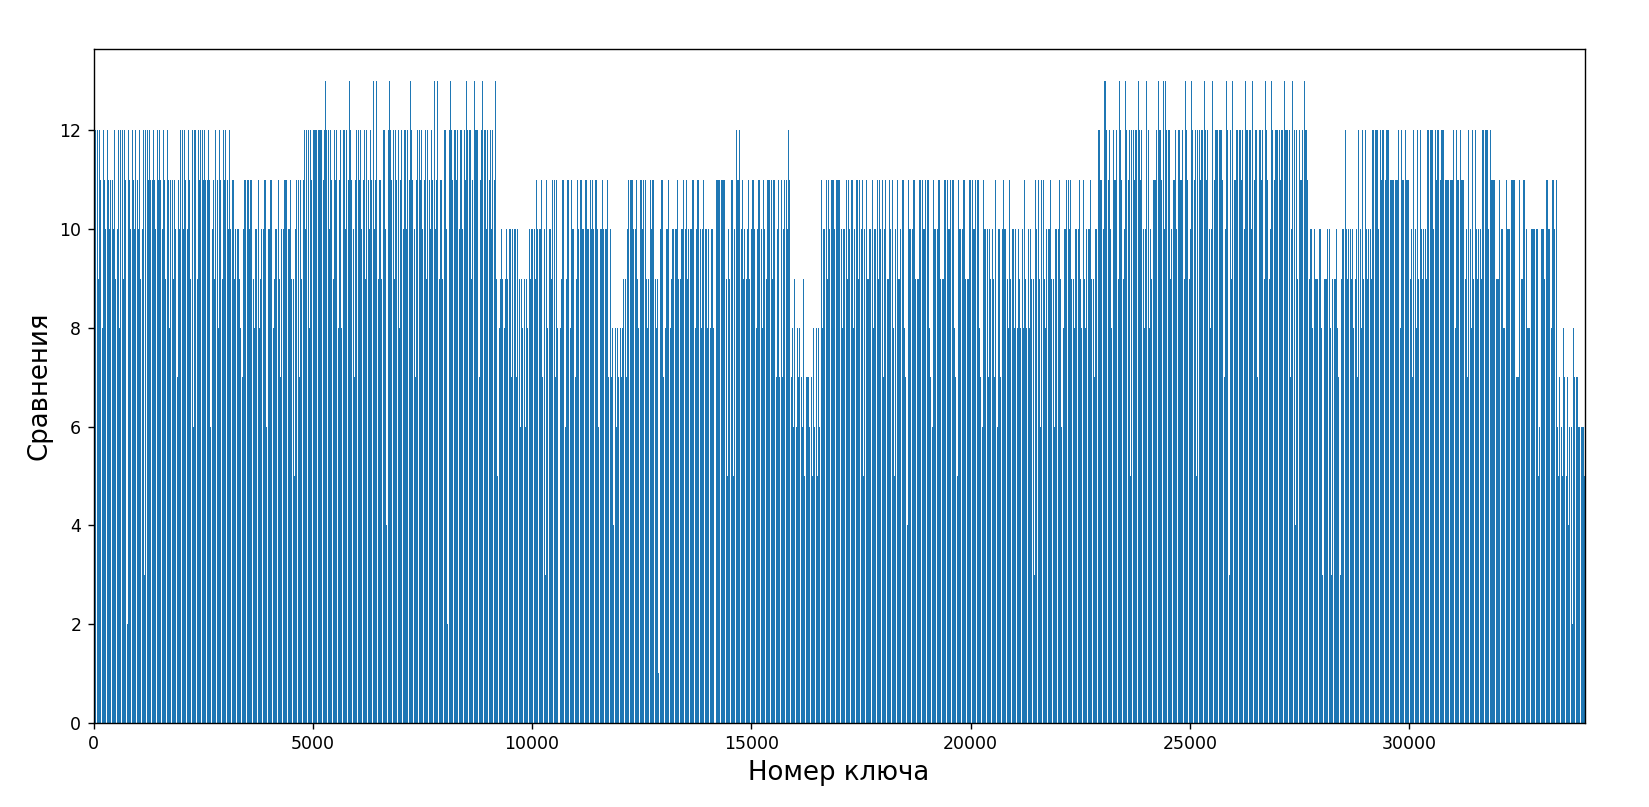
\includegraphics[width=0.8\linewidth]{img/seg_keys}
			\caption{Число сравнений для нахождения частотным анализом.}
			\label{img:freq}
		\end{center}
	\end{figure}
	
	Как и в случае с бинарным поиском, не наблюдается явной зависимости числа сравнений для поиска элемента от его значения. В связи с этим, стоит так же упорядочить элементы по числу сравнений и построить вторую гистограмму.

	\begin{figure}[H]
		\begin{center}
			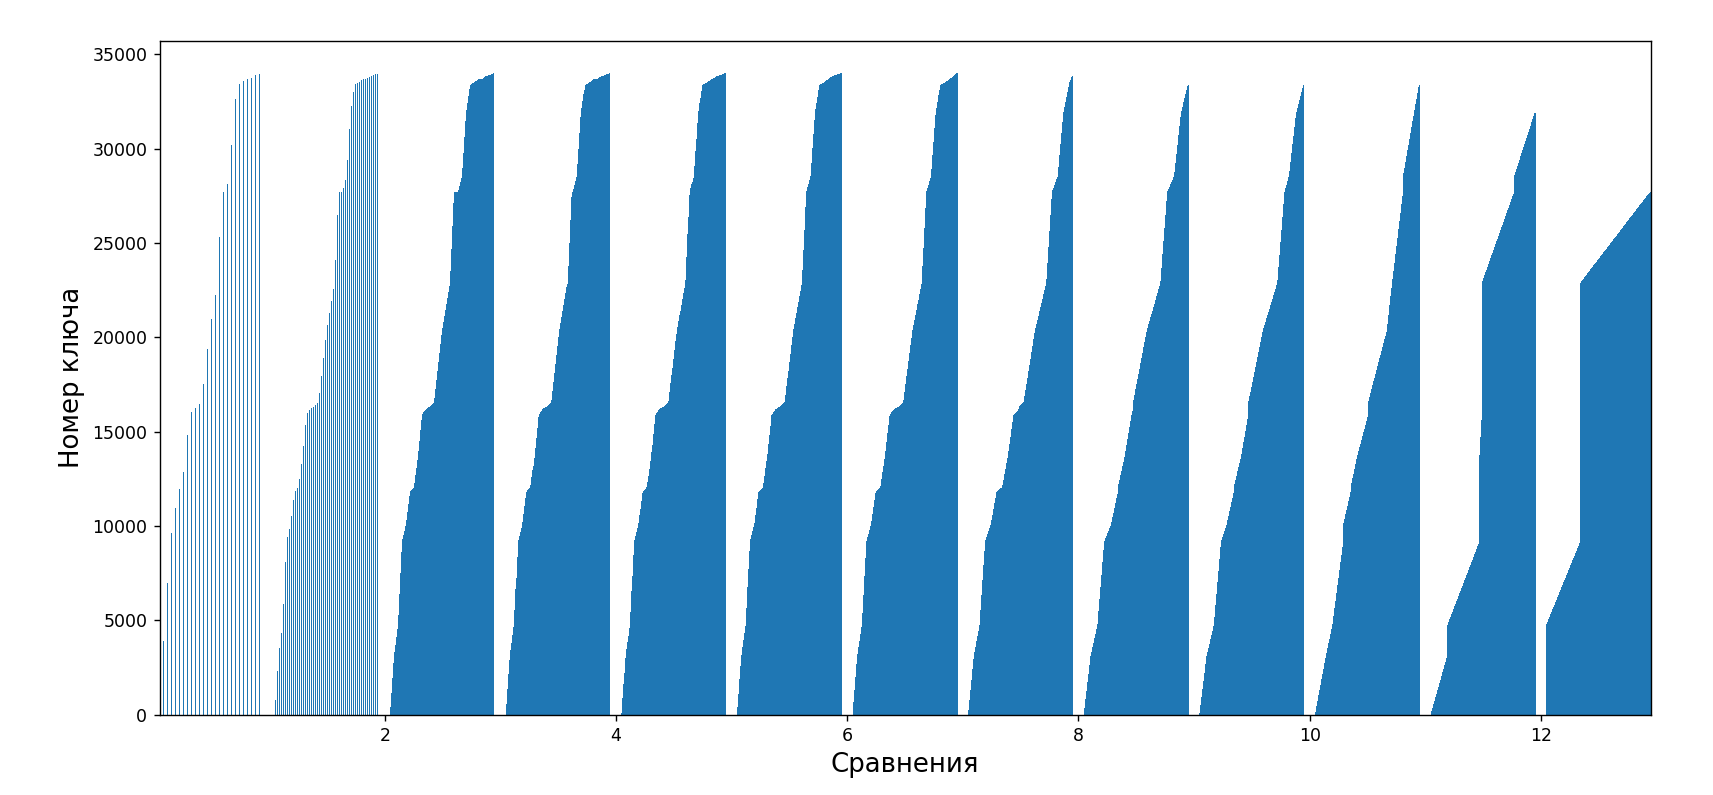
\includegraphics[width=0.8\linewidth]{img/seg_comp}
			\caption{Число сравнений для нахождения частотным анализом по убыванию.}
			\label{img:freq_sorted}
		\end{center}
	\end{figure}
	
	\section{Вывод}
	Исходя из полученных данных, можно сделать вывод, что алгоритм поиска в словаре, использующий частотный анализ, является боле эффективным, чем алгоритм полного перебора лишь в ряде случаев, в остальных же, он является менее эффективным, в связи с использованием сегментации и бинарным поиском внутри сегмента.
	
	Отдельно надо отметить, что алгоритм бинарного поиска требует меньшего числа сравнений, в связи с чем является более эффективным, чем алгоритм с частотным анализом. Однако алгоритм бинарного поиска требует сортировки всего входного массива, что, в среднем случае имеет сложность $O(nlog(n))$, в связи с чем алгоритм бинарного поиска становится менее эффективным, чем алгоритм частотного анализа, сортирующий данные по сегментам.
	
	\newpage
	\addcontentsline{toc}{chapter}{Заключение}
	\chapter*{Заключение}
	Задачами данной работы являлись:
	
	\begin{itemize}
		\item изучить существующие алгоритмы поиска по словарю;
		\item определить требования к программе для решения задачи поиска по словарю;
		\item описать структуры данных;
		\item определить классы эквивалентности для тестирования;
		\item определить тестовые данные;
		\item осуществить выбор средств реализации;
		\item реализовать алгоритмы программно;
		\item исследовать время работы алгоритмов;
		\item сравнить время работы алгоритмов и сделать соответствующие выводы.
	\end{itemize}

	Все задачи были выполнены в ходе работы.

	Первым этапом было дано определение поиску по словарю.

	Затем были исследованы существующие алгоритмы решения задачи поиска и были выбраны 3
	алгоритма для сравнения:
	\begin{itemize}
		\item алгоритм полного перебора;
		\item алгоритм двоичного поиска;
		\item алгоритм частотного анализа.
	\end{itemize}

	Далее были определены требования к программе, составлены блок-схемы алгоритмов и произведена разработка на языке Python.

	В итоге было произведено исследование поиска по словарю с помощью трех алгоритмов.
	
	По результатам исследования можно сделать вывод, что алгоритм поиска в словаре, использующий частотный анализ, является боле эффективным, чем алгоритм полного перебора лишь в ряде случаев, в остальных же, он является менее эффективным, в связи с использованием сегментации и бинарным поиском внутри сегмента.
	
	\addcontentsline{toc}{chapter}{Список литературы}
	\bibliographystyle{utf8gost705u}
	\bibliography{report_6}
\end{document}